%! TEX root = ../mersenne.tex
\section{Introduction}
Polynomial hashing using Mersenne primes is well-known for being faster
than polynomial hashing using arbitrary primes. Here we argue that
uniform hash values from a Mersenne prime field with prime $p=2^b-1$
can largely be treated as uniform $b$-bit strings, that is, we can use
the tool box of very simple and efficient tricks for uniform
$b$-bit strings.

From $[2^b]$ we are missing $p$, the all \texttt1s value, but a careful analysis shows that this has only minor effect on the quality of the outcome.
To put our results in perspective, suppose we were hashing $n$ keys uniformly into $b$-bit strings.
The probability that any of them hash to $p=2^b-1$ is at most $n/p$.
This mean the total variation between the two distributions is $n/p$ and any error probability we might have proved assuming uniform $b$-bit hash values is off by at most $n/p$.
%This may be good if $p/n$ is sufficiently large.
\emph{In contrast, our analysis yields errors of $n/p^2$ or less!}
This allows good error bounds even as we set $p$ close to $n$, which again means that half the word operations can saved.

Many of the ideas presented here would not apply at all if we had a prime $2^b-a$ with $a>1$, e.g., $a=3$, so our work is very particular to Mersenne primes.
Primes on the form $2^b-a$ with $a>1$ are known as Pseudo-Mersenne Primes~\cite{van2014encyclopedia}, and are often sometimes used when a Mersenne prime of a reasonable magnitude isn't available.
Supplementing our main analysis, we provide a new algorithm for division and hashing with such numbers, which improves upon classical cryptographic work by Crandall~\cite{crandall1992method}.

While hashing with Mersenne primes has been used for more than 40 years by anyone who, for k>2, wanted to implement k-universal hashing efficiently using standard portable code, we believe we are the first to notice the special advantages of having hash values that are uniform in a Mersenne prime field rather than any other prime field. Essentially our new kind of analysis shows that we can reduce errors from $n/p$ to $n/p^2$.
This means that we for a desired error can reduce the bit-length of the primes to less than half. This saves not only space. It typically means that we can speed up the multiplications with at least a factor 2.

Hashing is often used in the sketching of high volume data streams, such as traffic through an Internet router, and then this speed is critical to keep up with the stream.

\begin{figure}

   \centering
   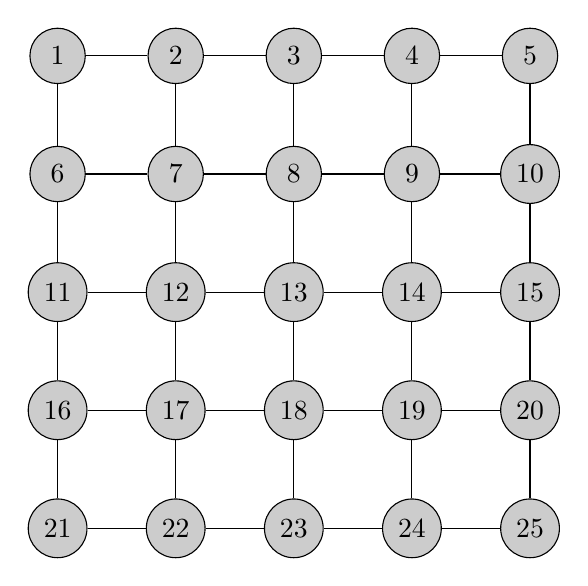
\begin{tikzpicture}[darkstyle/.style={circle,draw,fill=gray!40,minimum size=20}]
     \foreach \x in {0,...,4}
       \foreach \y in {0,...,4} 
          {\pgfmathtruncatemacro{\label}{\x - 5 *  \y +21}
          \node [darkstyle]  (\x\y) at (1.5*\x,1.5*\y) {\label};} 

     \foreach \x in {0,...,4}
       \foreach \y [count=\yi] in {0,...,3}  
         \draw (\x\y)--(\x\yi) (\y\x)--(\yi\x) ;

   \end{tikzpicture}
   \caption{test}
   \label{fig:bits}
\end{figure}

\subsection{Polynomial hashing using Mersenne primes}



The k-universal hashing with a polynomial uses O(k) space and O(k) time
to compute the hash value of a key. Siegel \cite{Siegel04} has proved that if we want k universal hashing in time t<k, then we need to use space $u^{1/t}$.
Such tabulation based methods are useful in many contexts (see survey \cite{Thorup17} , but not if we need small space. 

A classic example where constant space hash functions are needed is in static two-level hash functions \cite{FKS84}. To store n keys with constant access time, they n second level hash tables, each with its own  hash function.

Another example is small sketches such as the count sketch cite{XXX} discussed in this paper. Here we may want to store the hash function as part of the sketch, e.g., to query the value of a given key.


\subsubsection{Preliminaries: The classical implementation}
The classic definition of $k$-universal (or $k$-independent) hashing
goes back to Carter and Wegman \cite{wegman81kwise}.
\begin{definition}
   A random hash function $h:U\to R$ is $k$-universal if for any $j\leq k$
   distinct keys $x_0,\ldots,x_{j-1}$, the vector
   $(h(x_0),\ldots,h(x_{j-1}))$ is uniformly distributed in $R^j$. This
   is equivalent to saying that each $h(x_i)$ is uniform in $R$ and that
   all the $h(x_i)$ are independent of each other.
\end{definition}
The classic example of $k$-universal
hash function is uniformly random degree-$(k-1)$ polynomial over a prime field
$\Z_p$, that is, we pick a uniformly random vector
$\vec a=(a_0,\ldots,a_{k-1})\in \Z_p^k$ of $k$ coefficients, and define
$h_{\vec a}:[p]\to[p]$,
\footnote{ We use the notation $[s]=\{0,\ldots,s-1\}$.  }
   by 
\[h_{\vec a}(x)=\sum_{x\in[k]}a_i x^i \mod p.\]
%
Generally, we are given a key domain $[u]$ and a smaller range $[r]$ for the hash values.
It is natural to define
$h^r_{\vec a}:[u]\to[r]$ by
\[h^r_{\vec a}(x)=h_{\vec a}(x)\bmod r.\]
Assuming $p\geq \max\{u,r\}$, the hash values of $k$ distinct keys remain independent,
while staying as close as possible to the uniform distribution on $[r]$.
(This will turn out to be very important.)

In terms of speed, the main bottleneck in the above approach is the mod operations.
If we assume $r=2^\ell$, the $\bmod r$ operation above can be replaced by a binary AND: $x \bmod r = x \andtt r-1$.
In the same vein, an old idea by 
Carter and Wegmen \cite{carter77universal} is to use a
Mersenne prime for $p=2^b-1$,\footnote{e.g., $p=2^{61}-1$ for hashing 32-bit keys or
$p=2^{89}-1$ for hashing 64-bit keys.}
to speed up the computation of the $\mod p$ operations.
The point is that
\begin{equation}
   y \bmod (2^b-1)
   \equiv (y\bmod 2^{b}) + \floor{y/2^b}
   \equiv (y \andtt p) + (y \rs b)
   \pmod {p}.
   \label{eq:Mersenne}
\end{equation}
%This leads to efficient computations because 
%\[y\bmod 2^{b}=y\andtt p\quad\textnormal{and}\quad\floor{y/2^b}=y\rs b.\]
Again allowing us to use the very fast bit-wise {\sc and} ($\andtt$) and the right-shift ($\rs$),
instead of the expensive modulo operation.


\vspace{.5em}

The above completes our description of how Mersenne primes are
normally used for fast computation of $k$-universal hash functions.
We show an implementation in \cref{alg:Mersenne} with one further improvement:
By assuming that $p=2^b-1\geq 2u-1$
(which is automatically satisfied in the typical case where $u$ is a power
of two, e.g., $2^{32}$ or $2^{64}$)
we can get away with only testing a possible off-by-one in \cref{eq:Mersenne} once, rather that at every loop.

\begin{algorithm}
   \caption{
      For $x\in [u]$, prime $p=2^b-1\geq 2u-1$,
      and $\vec a=(a_0,\ldots,a_{k-1})\in[p]^k$,
      compute $h_{\vec a}(x)=\left(\sum_{i\in[q]}a_i x^i\right)\bmod p$
   }\label{alg:Mersenne}
   \begin{algorithmic}[1]
      \State $y\gets a_{k-1}$
      \For{$i=q-2,\ldots,0$}
      \Comment{$\quad y<2p$}

      \State $y\gets y*x+a_i$
      \Comment{$\quad y<2p(u-1)+(p-1)<(2u-1)p\leq p^2$}

      \State $y\gets (y\andtt p)+(y\rs b)$
      \Comment{$\quad y<p+p^2/2^b<2p$}
      \EndFor
      \If{$y\geq p$}
      \State $y\gets y-p$
      \EndIf
      \State \Return $y$
   \end{algorithmic}
\end{algorithm}


In \Cref{subsec:intro-division} we will give one further improvement to \Cref{alg:Mersenne}.
Mostly the description above is a fairly standard description of state-of-the-art hashing.
\footnote{We note that $k=2$, we do have the fast multiply-shift scheme of Dietzfelbinger~\cite{dietzfel96universal}, that directly gives 2-universal
hashing from $b$-bit strings to $\ell$-bit strings, but for $k>2$,
there is no faster method that can be implemented in with portable code
in a standard programming language like C.}

We stress that while this is a particularly fast implementation of Mersenne prime hashing, the main novelty of the paper will be in the analysis.
In particular 

The main point of this paper is our note from before, that the values hashed to $[r]$ are not completely uniform, as they would have been if $p=2^b$ was a prime.
It turns out that with a novel analysis, bits from Mersenne primes are actually
%$k$-universal hash values from $[2^b-1]$ can be
almost as good as if
they were uniformly distributed $b$-bit strings (we are only missing
the all \texttt{1}s value $2^b-1$). 





\subsubsection{Good bucketing with powers of two}\label{sec:power-of-two}
As a first trivial illustration of the quality that we get using a
Mersenne prime $p=2^b-1$, consider the case mentioned above where we
want hash values in the range $[r]$ where $r=2^\ell$ is a power of
two. We will often refer to the hash values in $[r]$ as buckets so
that we are hashing keys to buckets. Avoiding a degenerate case, we
assume $r>1$. In particular this implies that $r$ does not divide our
prime $p$.

We assume a $k$-universal hash function $h:[u]\to[p]$, e.g.,
the one from \Cref{alg:Mersenne}. To get hash values in $[r]$,
we defined $h^r:[u]\to[r]$ by
\[h^r(x)=h(x)\bmod r=h(x)\andtt (r-1).\]
As discussed previously, the hash values of up to $k$ distinct keys remain
independent with $h^r$. The issue is that hash values from 
$h^r$ are not quite uniform in $[r]$.

Recall that for any key $x$, we have $h(x)$ uniformly distributed in $[2^b-1]$.
This is the uniform distribution on $b$-bit strings except that we are
missing $p=2^b-1$. Now $p$ is the all \texttt{1}s, and 
$p \bmod r = p\andtt (r-1) = r-1$. Therefore, for any 
any $i<r-1$,
\begin{equation}\label{eq:coll-ell<r-1}
   \Pr[h^r(x)=i]=\lceil p/r\rceil/p=((p+1)/r)/p
   =(1+1/p)/r\textnormal,
\end{equation}
while 
\begin{equation}\label{eq:coll-ell=r-1}
   \Pr[h^r(x)=r-1]=\lfloor p/r\rfloor/p=((p+1-r)/r)/p
   =(1-(r-1)/p)/r.
\end{equation}
Thus $\Pr[h^r(x)=i]\leq (1+1/p)/r$ for all $i\in[r]$. This upper-bound
only has a relative error of $1/p$ from the uniform $1/r$. For
comparison, if we had used a prime of the form $p=2^b-a$ and $a<r$, then
we would only get an upper bound of $(1+a/p)/r$. Below we return
to a Mersenne prime $p=2^b-1$

Combining \req{eq:coll-ell<r-1} and \req{eq:coll-ell=r-1} with
pairwise independence, for any distinct keys $x,y\in [u]$, we show that the
collision probability is bounded
\begin{equation}\begin{split}  
   \Pr[h^r(x)=h^r(y)]
      =(r-1)((1+1/p)/r)^2+((1-(r-1)r/p)/r)^2
      %\\&= \frac{r +(r^2-r)/p^2}{r^2}
      =(1+(r-1)/p^2)/r
      %\\& <(1+r/p^2)/r
   %.\label{eq:coll}
\end{split}\end{equation}
We note that relative error $r/p^2$ is small as long as $p$ is
large.

\paragraph{Selecting arbitrary bits from the hash value}
Interestingly, the above analysis holds no matter which $\ell$ bits we
use when mapping the hash values from $[2^b-1]$ to $[2^\ell]$.  Let
$\mu:[2^b]\to[2^\ell]$ be any map defined by selecting $\ell$ bits
from a $b$-bit string. Above we used
$\mu(y)=y\bmod 2^\ell=y\andtt  (2^\ell-1)$,
selecting the $\ell$ least significant bits, but we could
also use $\mu(y)=\floor{y/2^{b-\ell}}=y\rs (b-\ell)$ selecting
the $\ell$ most significant bits. The basic point is that a uniform
distribution on $[2^b]$ maps to a uniform distribution on
$[2^\ell]$. We are only missing the all \texttt1s value $p=2^b-1$ which maps to $2^\ell-1$
regardless of which $\ell$ bits we select, so our equations
\req{eq:coll-ell<r-1}--\req{eq:coll} hold no matter which $\ell$
bits we select for $h^r$.

The fact that it doesn't matter which $\ell$ bits we select is only
true because we use a Mersenne prime $p=2^b-1$. Suppose we used some
other $b$-bit prime $p=2^b-a$ where $2^{b-\ell}<a<2^{b-1}$. If we
select the $\ell$ most signifant bits, then $0$ elements from $[p]$
map to $2^\ell-1$ while $2^{b-\ell}$ elements from $[p]$ map to $0$. However,
with the $\ell$ least significant bits, we have $\floor{p/2^\ell}$ or
$\ceil{p/2^\ell}$ elements from $[p]$ mapping to each element in
$[2^\ell]$, so the maximal difference is 1.


\subsection{Two-for-one hash functions in second moment estimation}
In this section we discuss how we can get several hash functions for
the price of one, and apply the idea to second moment estimation using
count sketches \cite{charikar04count-sketch}.

Suppose we had a $k$-universal hash function into $b$-bit strings.
We note that using standard programming languages such as C, we have
no simple and efficient method computing such hash
functions when $k>2$. However, later we will argue that polynomial
hashing using a Mersenne prime $2^b-1$ delivers a better-than-expected
approximation.

Let $h:U\to [2^b]$ be $k$-universal. By definition this
means that if we have $j\leq k$ distinct keys $x_1,\ldots,x_j$, then
$(h(x_1),\ldots,h(x_j))$ is uniform in $[2^b]^j\equiv [2]^{bj}$,
so this means that \emph{all} the bits in $h(x_1),\ldots,h(x_j)$ are
independent and uniform. We can use this to split our $b$-bit hash
values into smaller segments, and sometimes use them as if
they were the output of independently computed hash functions.
We illustrate this idea below in the context of the second moment estimation.

\subsubsection{Second moment estimation}
We now review the second moment estimation of streams based on count
sketches \cite{charikar04count-sketch} (which are based on the
celebrated second moment AMS-estimator from \cite{alon96frequency})

The basic set-up is as follows.  For keys in $[u]$ and integer values in $\Z$, we are given a stream of key/value $(x_0,\Delta_0),\ldots, (x_{n-1},\Delta_{n-1})\in [u]\times\Z$. The
total value of key $x\in[u]$ is
\[f_x=\sum_{i\in[n],x_i=x} \Delta_i.\]
We let $n\leq u$ be  the number of non-zero values
$f_x\neq 0$, $x\in [u]$. Often $n$ is much smaller than $u$.
We define the $m$th moment to be the $m$-norm to $m$th power,
$F_m^m = \sum_{x\in [u]}f_y^m$. The goal here is to
estimate the second moment $F_2^2 = \sum_{x\in [u]}f_x^2$. 

\begin{algorithm}
   \caption{\label{alg:count-sketch} Count Sketch. Uses a
      vector/array $C$ of $r$ integers and two independent
      4-universal hash functions $i:[u]\to[r]$ and $s:[u]\to\{-1,1\}$.
   .}
   \begin{description}
      \item[Initialize] For $i\in[t]$, set $C[i]\gets 0$.
      \item[Process$(x,\Delta)$] $C[i(x)]\gets C[i(x)]+s(x) \Delta$. 
      \item[Output] $X=\sum_{i\in[t]} C[i]^2$.
   \end{description}
\end{algorithm}
The standard analysis \cite{charikar04count-sketch} shows that 
\begin{align}
   \E[X]&= \| f\|_2^2 \label{eq:E-F2}\\
   \Var[X]&=2(\| f\|_2^4 - \| f\|_4^4)/r<2\| f\|_2^4/r \label{eq:V-F2}
\end{align}
By Chebyshev's inequality, this implies
\[\Pr[|X-\| f\|_2^2|\geq \eps \| f\|_2^2]\leq \Var[X]/(\eps \| f\|_2^2)^2<
2/(k\eps^2).\]
With $t=8/\eps^2$, the error probability is below 1/4.
To
reduce the error probability, we can use the standard trick of
making $r$ independent experiments
and return the median estimate. Using Chernoff bounds, the probability
that the median deviates by more than $\eps \| f\|_2^2$ is bounded by
$\exp(-r/12)$.

\subsubsection{Two-for-one hash functions with \texorpdfstring{$b$}{b}-bit hash values}
As the count sketch is described above,
it uses two independent 4-universal hash functions
$i:[u]\to[r]$ and $s:[u]\to\{-1,1\}$, but 4-universal hash functions
are generally slow to compute, so, aiming to save roughly a factor 2
in speed, a tempting idea is to compute them both using a single hash
function.

The analysis behind \req{eq:E-F2} and \req{eq:V-F2} does not quite
require $i:[u]\to[r]$ and $s:[u]\to\{-1,1\}$ to be independent.
It suffices that the hash values are uniform and that for any
given set of $j\leq 4$ distinct keys $x_1,\ldots,x_j$, the $2j$ hash
values $i(x_1),\ldots,i(x_j),s(x_1),\ldots,s(x_j)$ are independent.
A critical step in the analysis is that if
$A$ depends on $i(x_1),\ldots,i(x_j),s(x_2),\ldots,s(x_j)$, but
not on $s(x_1)$, then
\begin{equation}\label{eq:E-0}
  \E[s(x_0) A] = 0 .
\end{equation}
This follows because $\E[s(x_1)]=0$ by uniformity of $s(x_1)$ and because $s(x_1)$ is independent of $A$.


Assuming that $t=2^\ell$ is a power of two, we can easily construct
$i:[u]\to[t]$ and $s:[u]\to\{-1,1\}$ using a single $4$-universal
hash function $h:[u]\to[2^b]$ where $b>\ell$. Recall that all the bits in
$h(x_1),\ldots,h(x_4)$ are independent. We can therefore use the
$\ell$ least significant bits of $h(x)$ for $i(x)$ and the most
significant bit of $h(x)$ for a bit $a(x)\in[2]$, and finally set
$s(x)=1-2a(x)$. It is then easy to show that if $h$ is $k$-universal
than $h$ satisfies \cref{eq:E-0}.
\begin{algorithm}
   \caption{For key $x\in [u]$, compute $i(x)=i_x\in[2^\ell]$ and
      $s(x)=s_x\in\{-1,+1\}$,\rule{5ex}{0ex}
   using $h:[u]\to [2^b]$ where $b>\ell$.}
   \label{alg:h-and-s}
   $h_x\gets h(x)$\hfill $\rhd\quad h_x$ uses $b$ bits\\
   $i_x\gets h_x \andtt (2^\ell-1)$\hfill $\rhd\quad i_x$ gets $\ell$ least significant
   bits of $h_x$\\
   $a_x\gets h_x\rs (b-1)$\hfill $\rhd\quad a_x$ gets the most significant bit of $h_x$\\
   $s_x\gets 1-2a_x$ \hfill $\rhd\quad a_x\in[2]$ is converted to a sign $s_x\in\{-1,+1\}$
\end{algorithm}
% \begin{lemma}\label{lem:b-bit-hashing} Suppose $h:[u]\to[2^b]$ is $k$-universal. Let
%    $i:[u]\to[2^\ell]$ and
%    $s:[u]\to\{-1,1\}$ be constructed from $h$ as described in Algorithm \ref{alg:h-and-s}. Then $h$ and $s$ are both $k$-universal. Moreover, for
%    any $j\leq k$ distinct keys $x_1,\ldots,x_j$, the $2j$ hash
%    values $i(x_1),\ldots,i(x_j),s(x_1),\ldots,s(x_j)$ are independent.
%    In particular, if $A$ depends on
%    $i(x_1),\ldots,i(x_j),s(x_2),\ldots,s(x_j)$, but not on $s(x_1)$, then
%    \begin{equation}\label{eq:E-0}
%       \E[s(x_1)A]=0
%    \end{equation}
% \end{lemma}
Note that Algorithm \ref{alg:h-and-s} is well defined as long as 
$h$ returns a $b$-bit integer. However, \cref{eq:E-0} requires
that $h$ is $k$-universal into $[2^b]$, which in particular implies that
the hash values are uniform in $[2^b]$.


\subsubsection{Two-for-one hashing with  Mersenne primes}\label{sec:two-for-one}
Above we discussed how useful it would be with $k$-universal hashing
mapping uniformly into $b$-bit strings. The issue was that the lack of
efficient implementations with standard portable code if
$k>2$. However, when $2^b-1$ is a Mersenne prime $p\geq u$, then we do
have have the efficient computation from Algorithm \ref{alg:Mersenne}
of a $k$-universal hash function $h:[u]\to[2^b-1]$. The hash values
are $b$-bit integers, and they are uniformly distributed, except that
we are missing the all \texttt{1}s value $p=2^b-1$. We want to
understand how this missing value affects us if we try to split the
hash values as in Algorithm \ref{alg:h-and-s}. Thus, we assume a
$k$-universal hash function $h:[u]\to[2^b-1]$ from which we construct
$i:[u]\to[2^\ell]$ and $s:[u]\to\{-1,1\}$ as
described in Algorithm \ref{alg:h-and-s}. As usual, we assume $2^\ell>1$.
Since $i_x$ and $s_x$ are
both obtained by selection of bits from $h_x$, we know from Section
\ref{sec:power-of-two} that each of them have close to uniform
distributions. However, we need a good replacement for \req{eq:E-0}
which besides uniformity, requires $i_x$ and $s_x$ to be independent,
and this is certainly not the case.

Before getting into the analysis, we argue that we really do get two
hash functions for the price of one. The point is that our efficient
computation in Algorithm \ref{alg:Mersenne} requires that we use a
Mersenne prime $2^b-1$ such that $u\leq 2^{b-1}$, and this is even if
our final target is to produce just a single bit for the sign function
$s:[u]\to\{-1,1\}$. We also know that $2^\ell<u$, for otherwise we
get perfect results implementing $i:[u]\to[2^\ell]$ as the identifty
function (perfect because it is collision free).  Thus we can assume
$\ell<b$, hence that $h$ provides enough bits for both $s$ and $i$.


We now consider the effect of the hash values from $h$ being uniform
in $[2^b-1]$ instead of in $[2^b]$. Suppose we want to compute the
expected value of an expression $B$ depending only on the independent
hash values $h(x_1),\ldots,h(x_j)$ of $j\leq k$ distinct keys
$x_1,\ldots,x_j$.

Our generic idea is to play with the distribution of $h(x_1)$ while
leaving the distributions of the other independent hash values
$h(x_2)\ldots,h(x_j)$ unchanged, that is, they remain uniform in
$[2^b-1]$. We will consider having $h(x_1)$ uniformly distributed in
$[2^b]$, denoted $h(x_1) \sim \unif[2^b]$, but then we later have to
subtract the ``fake'' case where $h(x_1)=p=2^b-1$.  Making the
distribution of $h(x_1)$ explicit, we get
\begin{equation}\begin{split}
  \E_{h(x_1) \sim \unif[p]}[B]&=\sum_{y\in[p]}\E[B \mid h(x_1)=y]/p
  =\sum_{y\in[2^b]}\E[B \mid h(x_1)=y]/p - \E[B \mid h(x_1)=p]/p \\
  &=\E_{h(x_1) \sim \unif[2^b]}[B](p+1)/p - \E[B \mid h(x_1)=p]/p.\label{eq:play-with-dist}
\end{split}\end{equation}
Let us now apply this idea our situation where $i:[u]\to[2^\ell]$ and
$s:[u]\to\{-1,1\}$ are constructed from $h$ as described in Algorithm
\ref{alg:h-and-s}. We will prove
\begin{lemma}\label{lem:remove-si}  Consider distinct keys $x_1,\ldots,x_j$, $j\leq k$ and an expression $B=s(x_1)A$ where $A$
   depends on $i(x_1),\ldots,i(x_j)$ and $s(x_2),\ldots,s(x_j)$ but not
   $s(x_1)$. Then
   \begin{equation}\label{eq:remove-si}
      \E[s(x_1)A]=\E[A\mid i(x_1)=2^\ell-1]/p.
   \end{equation}
\end{lemma}
\begin{proof}
When $h(x_1) \sim \unif[2^b]$, then $s(x_1)$ is uniform
in $\{-1,+1\}$ and independent of $i(x_1)$. The remaining
$(i(x_i),s(x_i))$, $i>1$, are independent of $s(x_1)$ because they
are functions of $h(x_i)$ which is independent of $h(x_1)$, so
we conclude that 
\[\E_{h(x) \sim \unif[2^b]}[s(x_1)A]=0\]
Finally, when $h(x_1)=p$, we get $s(x_1)=-1$ and $i(x_1)=2^\ell-1$, 
so applying \req{eq:play-with-dist}, we conclude
that 
\[\E[s(x_1)A] = -\E[s(x_1) A \mid h(x_1) = p]/p = \E[A \mid i(x)=2^\ell-1]/p.\]
\end{proof}
Above \req{eq:remove-si} is our replacement for \req{eq:E-0}, that is,
when the hash values from $h$ are uniform in $[2^b-1]$ instead of
in $[2^b]$, then $\E[s(x_1)B]$ is reduced by $\E[B \mid i(x)=2^\ell-1]/p$.
For large $p$, this is a small additive error. Using this in a careful
analysis, we will show that our fast second moment estimation 
based on Mersenne primes performs almost perfectly:

\begin{theorem}\label{thm:h-and-s-p}
   Let $r>1$ and $u>r$ be powers of two and let $p=2^b-1>u$ be a
   Mersenne prime.
   Suppose with have a $k$-universal hash function $h:[u]\to[2^b-1]$, e.g.,
   generated using Algorithm \ref{alg:Mersenne}. Suppose
   $i:[u]\to[r]$ and
   $s:[u]\to\{-1,1\}$ are constructed from $h$ as described in
   Algorithm \ref{alg:h-and-s}. Using this $i$ and $s$ 
   in the Count Sketch Algorithm \ref{alg:count-sketch}, the second moment 
   estimate $X=\sum_{i\in[k]} C_i^2$ satisfies:
   \begin{align}
      \E[X]=&F_2+(F_1^2-F_2)/p^2 < (1+n/p^2)\,F_2\textnormal,\label{eq:E-F2-p}\\
      \Var[X]&< 2(F_2^2-F_4)/r+F_2^2 (2.33+4 n/r)/p^2<2F_2^2/r.\label{eq:V-F2-p}
   \end{align}
\end{theorem}
The difference from \req{eq:E-F2} and \req{eq:V-F2} 
is negligible when $p$ is large. Theorem \ref{thm:h-and-s-p} will be
proved in Section \ref{sec:analysis-two-for-one}.


\subsection{Arbitrary number of buckets}\label{sec:most-uniform}
We now consider the general case where we want to hash into a set of buckets $R$ whose size is not a power of two.
Suppose we have a $2$-universal hash function $h:U\to Q$.
We will compose $h$ with a map $\mu:Q\to R$, and use $\mu\circ h$ as a hash function from $U$ to $R$.
Let $q=|Q|$ and $r=|R|$.
We want the map $\mu$ to be \emph{most uniform} in the sense that for bucket $i\in R$, the number of elements from $Q$ mapping to $i$ is either $\floor{q/r}$ or $\ceil{q/r}$.
Then the uniformity of hash values with $h$ implies for any key $x$ and bucket $i\in R$ \[\floor{q/r}/q\leq \Pr[\mu(h(x))=i]\leq \ceil{q/r}/q.\]
Below we typically have $Q=[q]$ and $R=[r]$.
A standard example of a most uniform map $\mu:[q]\to[r]$ is $\mu(x)=x\bmod r$ which the one used above when we defined $h^r:[u]\to[r]$, but as we mentioned before, the modulo operation is quite slow unless $r$ is a power of two.

Another example of a most uniform map $\mu:[q]\to[r]$ 
is $\mu(x)=\floor{xr/q}$,
which is also quite slow in general, but if $q=2^b$ is a power of two,
it can be implemented as $\mu(x)=(xr)\rs\,b$ where 
$\rs$ denotes right-shift. This would be yet another advantage 
of of having $k$-universal hashing into $[2^b]$.\todo{Add comment about it being efficient for Mersenne aswell using our result!}

Now, our interest is the case where $q$ is a Mersenne prime $p=2^b-1$. We want
an efficient and most uniform map $\mu:[2^b-1]$ into any given $[r]$.
Our simple solution is to define
\begin{equation}\label{eq:most-uniform}
   \mu(x)=\floor{(x+1)r/2^b}=((x+1)r)\rs b.
\end{equation}
Lemma \ref{lem:most-uniform} (iii) below 
states that \req{eq:most-uniform} indeed
gives a most uniform map. 
\begin{lemma}\label{lem:most-uniform} Let $r$ and $b$ be positive integers.
   %, and let $x\in [2^b-1]$.
   Then
   \begin{itemize}
      \item[(i)] $x\mapsto (xr)\rs\,b$ is a most
         uniform map from $[2^b]$ to $[r]$.
      \item[(ii)] $x\mapsto (xr)\rs\,b$ is a most
         uniform map from $[2^b]\setminus\{0\}=\{1,\ldots,2^b-1\}$ to $[r]$.
      \item[(iii)] $x\mapsto ((x+1)r)\rs \, b$ is a most
         uniform map from $[2^b-1]$ to $[r]$.
   \end{itemize}
\end{lemma}
\begin{proof}
   Trivially (ii) implies (iii). 
   The statement (i) is folklore and easy to prove, so we know that every
   $i\in[r]$ gets hit by $\floor {2^b/r}$ or $\ceil{2^b/r}$ elements from
   $[2^b]$. It is also clear that $\ceil{2^b/r}$ elements, including $0$,
   maps to $0$. To prove (ii), we remove $0$ from $[2^b]$, 
   implying that only
   $\ceil{2^b/r}-1$ elements map to $0$. For all positive integers $q$
   and $r$, $\ceil{(q+1)/r}-1=\floor{q/r}$, and we use this here with 
   $q=2^b-1$. It follows that all buckets from $[r]$ gets $\floor{q/r}$
   or $\floor{q/r}+1$ elements from $Q=\{1,\ldots,q\}$. If $r$ does
   not divide $q$ then $\floor{q/r}+1=\ceil{q/r}$, as desired. However,
   if $r$ divides $q$, then $\floor{q/r}=q/r$, and this
   is the least number of elements from $Q$ hitting any bucket in $[r]$. Then 
   no bucket from $[r]$ can get hit by more than $q/r=\ceil{q/r}$ 
   elements from $Q$. This completes the proof of (ii), and hence of (iii).
\end{proof}
We note that our trick does not work when $q=2^b-a$ for $a\geq 2$, that is,
using $x\mapsto ((x+a)r)\rs  b$, for in this general case, 
the number of elements hashing to $0$ is $\ceil {2^b/r}-a$, or $0$ if
$a\geq \floor {2^b/r}$.
One may try many other hash functions $(c_1 x r+ c_2 x+ c_3 r + c_4) \rs b$ similarly without any luck.
Our new uniform map from \req{eq:most-uniform} is thus very specific to Mersenne prime fields.
For general $a\ge 2$ we provide a scheme using two shifts in Section \ref{sec:division}.

We will see in Section \ref{sec:count-sketch-r} that our new uniform map
works very well in conjunction with the idea of splitting of hash values 
values from Section \ref{sec:two-for-one}.




\subsection{Even faster division and modulo with (Pseudo) Mersenne Primes}\label{subsec:intro-division}
%
\begin{algorithm}
   \caption{For Mersenne prime $p=2^b-1$ and $x< 2^{2b}$, computes
   \label{alg:div-simple}
   $y=x\bmod p$ and $z=\floor{x/p}$}
   \begin{algorithmic}
      \State $z \gets x+1 \rs b$,
      \State $z \gets z+x+1 \rs b$,
      %\State $y \gets x - (z \ls b) + z$.
      \State $y \gets (x + z) \andtt p $.
   \end{algorithmic}
\end{algorithm}
%
We even suggest a speed-up the computation of $\pmod p$ for Mersenne primes
$p=2^b-1$. The issue in Algorithm \ref{alg:Mersenne} is that
if-statement can be slow because of branch prediction.
From the standard Algorithm \ref{alg:Mersenne} this means that we can
replace the last three lines statements
\begin{algorithmic}
   \State $y \gets (y\andtt p)+(y\rs b)$
   \If{$y\ge p$}
      \State $y\gets y-p$
   \EndIf
\end{algorithmic}
with Algorithm \ref{alg:div-simple} above.

\vspace{1em}

In fact our Algorithm \ref{alg:div-simple} does much more than just division and modulo computation with Mersenne primes.
The full algorithm in Section \ref{sec:division} gives a fast, branch-less algorithm for division and modulo by any \emph{generalized} Mersenne Prime.
There are in general two kinds of such primes:
%Primes on the form $2^n-1$ are known as Mersenne primes, and are used all over Cryptography and Computer Science because they allow quicker algorithms than primes in general.
%This allows speeding up finite field arithmetic,
%since $c\bmod (2^n-1) = (c\bmod 2^n) + \lfloor k/n\rfloor$ if the value is smaller than $p=2^n-1$ (otherwise just subtract $p$.)

\begin{description}
   \item[Pseudo-Mersenne Primes]
      are primes on the form $2^n-c$, where is usually required that $c < 2^{\lfloor n/2\rfloor}$~\cite{van2014encyclopedia}.
      Crandal patented a method for working with Pseudo-Mersenne Primes in 1992~\cite{crandall1992method},
      why those primes are also sometimes called ``Crandal-primes''.
      The method was formalized and extended by Jaewook Chung and Anwar Hasan in 2003~\cite{chung2003more}.
      Our method, while simpler, has both stronger guarantees and better practical performance.
      We provide a comparison with the Crandal-Chung-Hansan method in Section 4.
      %also sometimes known as Crandall primes, are numbers on the form $2^n - c$ for a small odd $c$.
   \item[Generalized Mersenne Primes]
      also sometimes known as Solinas primes~\cite{Solinas2011}, are sparse numbers, that is $f(2^m)$ where $f(x)$ is a low-degree polynomial.
      Examples are the primes in NIST's document ``Recommended Elliptic Curves for Federal Government Use'':
         $p_{192} = 2^{192} - 2^{64} - 1$
      and
         $p_{384} = 2^{384}-2^{128}-2^{96}+2^{32}-1$.
      We simply note that Solinas primes are also Pseudo-Mersenne Primes, which allow a particularly fast multiplication with $c$.
      Hence our algorithms are also efficient for Generalised Mersenne primes.
\end{description}

Our generalized algorithm is shown in Algorithm \ref{alg:division-generalized}.
\begin{algorithm}
   \caption{For Pseudo-Mersenne prime $p=2^b-c$ and $x,m$ such that $x< (2^b/c)^m$, computes
      $v=\floor{x/p}$}
   \label{alg:division-generalized}
   \begin{algorithmic}[1]
      \Procedure{Divide}{x, n, c}
         \State $x' \gets x + c$
         \State $v \gets 0$
         %\For{$i\gets 1$ \textbf{to} $m$}
         \For{ $m$ times}
            \State $v \gets v * c + x'$
            \State $v \gets v \rs n$
         \EndFor
         %\EndFor
         \State \Return $v$
      \EndProcedure
   \end{algorithmic}
\end{algorithm}
The full proof of this is given in Theorem \ref{thm:simple-div} in Section \ref{sec:division}.

In the Crandall case $x\le 2^n$ and $c\le 2^{\floor n/2}$, as described by the Encyclopedia of Cryptography and Security~\cite{van2014encyclopedia}, we can let $m=2$, unroll the loop, and the algorithm runs in just two steps for a total of five operations:
   $$
   \left\lfloor\frac{x}{2^n-c}\right\rfloor
   = \left\lfloor\frac{\lfloor\frac{x'}{2^n}\rfloor c + x'}{2^n}\right\rfloor
      = (x' \rs n)*c + x' \rs n
   ,$$
   including $x'=x+c$.

%In fact our algorithm does something stronger, namely gives an efficient division algorithm for any number on the form $q-c$ where $q$ supports fast division.
The intuition for the algorithm is the expansion
\begin{align}
   \frac{x}{q-c}
   = \frac{x}{q}\sum_{i=0}^\infty \left(\frac{c}{q}\right)^i
   = x\frac{1+\frac{c+\frac{c^2 + \dots}{q}}{q}}{q}
   = \frac{\frac{\frac{\dots+x}{q}c+x}{q}c+x}{q},
\end{align}
however curiously we need to shift $x$ by $c$ to compensate for the rounding down.




%The proposed algorithm takes integers $n>c>0$ and $x$, and returns
%$\left\lfloor\frac{x}{2^n-c}\right\rfloor$.
%The algorithm performs two additions, a shift, and a multiplication with $c$ for each memory word occupied by $x$.
%Thus, in the case of Generalized Mersenne Primes with sparsity $k$, we can use a total of $3+k$ simple operations.


%Note that for many Pseudo Mersenne Primes, multiplication by $c$ can be replaced by a single shift, making the algorithm completely additions and shifts.

%Note that we use the same number of operations independent of $x$.


To compute modulo we use the fact that
\begin{align}
   x \bmod p
   = x - p\left\lfloor\frac{x}{p}\right\rfloor
   = x - (2^n - c)\left\lfloor\frac{x}{2^n-c}\right\rfloor,
\end{align}
which is only two additions, a shift, and a multiplication with $c$ on top of the division algorithm.
As $\floor{\frac{x}{p}} p \le x$ there is no danger of overflow.
An alternative method is to note
$x = \lfloor\frac{x}{p}\rfloor (2^n-c) + r$, so
$$x\bmod p = \left(x+c\left\lfloor\frac{x}{p}\right\rfloor \right) \bmod 2^n,$$
which is fast to compute using $(\andtt p)$.
This is the method applied in Algorithm \ref{alg:div-simple}.

%In the case $x\le 2^{2b}$ and $c=1$, we get the simplified Algorithm \ref{alg:div-simple} described above: $ \left\lfloor\frac{x}{2^n-1}\right\rfloor = (x+1 \rs n)+x+1 \rs n$.

\paragraph{Application to arbitrary number of buckets}
In Subsection~\ref{sec:most-uniform} we discussed how $\floor{\frac{h(x)r}{2^b-1}}$ provides a most uniform map from $[2^b-1]\to[r]$.
To avoid the division step, we instead considered the map
$\floor{\frac{(h(x)+1)r}{2^b}}$.
However, for primes on the form $2^b-c$, $c>1$ this approach doesn't provide a most-uniform map.
%
Instead we may use Algorithm \ref{alg:division-generalized} to compute
$$\left\lfloor\frac{h(x)r}{2^b-a}\right\rfloor$$
directly, getting a perfect most-uniform map.
(Another alternative was to pre-compute $q = \lfloor2^n/p\rfloor$ and take
$\floor{\frac{h(x)rq}{2^b}}$, however that requires larger words to store the product $h(x)rq$.)


\subsubsection{Related Algorithms}

Modulus computation by Generalized Mersenne primes is widely studied in the Cryptography community.
For example, four of the recommended primes in NIST's document ``Recommended Elliptic Curves for Federal Government Use'' are Generalized Mersenne.
Naturally, much work has been done on making computations with those primes fast.
Articles like ``Simple Power Analysis on Fast Modular Reduction with Generalized Mersenne Prime for Elliptic Curve Cryptosystems''~\cite{sakai2006simple}
give very specific algorithms such as Algorithm \ref{alg:solina}, for each of a number of well known such primes.

\begin{algorithm}
   \caption{Fast reduction modulo $p_{192} = 2^{192} - 2^{64} - 1$}
   \label{alg:solina}
   \begin{algorithmic}
      \State \textbf{input} $c \gets (c_5, c_4, c_3, c_2, c_1, c_0)$, where each $c_i$ is a 64-bit word, and $0 \le c < p^2_{192}$.
      \State $s_0 \gets (c_2, c_1, c_0)$
      \State $s_1 \gets (0, c_3, c_3)$
      \State $s_2 \gets (c_4, c_4, 0)$
      \State $s_3 \gets (c_5, c_5, c_5)$
      \State \textbf{return} $s_0 + s_1 + s_2 + s_3 \mod p_{192}$.
   \end{algorithmic}
\end{algorithm}

Division by Mersenne primes is a less common task, but a number of well known division algorithms can be specialized, such as 
 classical trial division, Montgomery's method and Barrett reduction.


%Montgomery method:
%\begin{align}
%   (aR\mod N)(bR\mod N) \mod N = (abR)R \mod N
%\end{align}
%We then need to remove the factor of $R$ by multiplying with its inverse $\mod N$.


The state of the art appears to be the modified Crandall Algorithm by Chung and Hasan~\cite{chung2006low}.
This algorithm, given in Algorithm \ref{alg:cch} modifies Crandall's algorithm~\cite{crandall1992method} from 1992 to compute division as well as modulo for generalized $2^n-c$ Mersenne primes.
\begin{algorithm}
   \caption{Crandall, Chung, Hassan algorithm. For $p=2^n-c$, computes $q, r$ such that $x = qp+r$ and $r<p$.}
   \label{alg:cch}
   \begin{algorithmic}[1]
      \Procedure{Divide}{x, n, c}
         \State $q_0 \gets x \rs n $
         \State $r_0 \gets x \andtt 2^n-1$
         \State $q \gets q_0, r\gets r_0$
         \State $i \gets 0$
         \While{$q_i>0$}
            \State $t \gets q_i*c$
            \State $q_{i+1} \gets t \rs n$
            \State $r_{i+1} \gets t \andtt {2^n -1}$
            \State $q\gets q+q_{i+1}$
            \State $r\gets r+r_{i+1}$
            \State $i\gets i+1$
         \EndWhile
         \State $t \gets 2^n-c$
         \While{$r\ge t$}
            \State $r\gets r-t$
            \State $q\gets q+1$
         \EndWhile
         \State\textbf{return} $q$
      \EndProcedure
   \end{algorithmic}
\end{algorithm}
The authors state that for $2n+\ell$ bit input, Algorithm \ref{alg:cch}
requires at most $s$ iterations of the first loop, if $c < 2^{((s-1)n-\ell)/s}$.
This corresponds roughly to the requirement $x < 2^n (2^n/c)^s$, similar to ours.

Unfortunately the algorithm ends up doing double work, by computing the quotient and remainder concurrently.
The algorithm also suffers from the extra while loop for ``cleaning up'' the computations after the main loop.



%No proof of correctness is given.
%The while loop condition is different.
%No guarantees on running time.
%The addition is different from ours.
%Doesn't add 1. Doesn't add $x$.
%Has that extra weird loop for fixing things in the end.
%So it actually has to do the $r$ computation?


Chung and Hasan also has an earlier, simpler algorithm from 2003~\cite{chung2003more},
but it appears to give the wrong result for many simple cases.
This appears to be because of a lack of the ``clean up'' while loop at the end of Algorithm \ref{alg:cch}.

%listed in Algorithm \ref{alg:cch2}.
%\begin{algorithm}\label{alg:cch2}
%   \caption{For $q=2^n-c$, computes $t, r$ such that $x = tq+r$ and $r<q$. (Broken.)}
%   \begin{algorithmic}[1]
%      \State $r \gets x$
%      \State $t \gets 0$
%      \While{$r > q$}
%         \State $A \gets r \rs n$
%         \State $B \gets r \andtt 2^n-1$
%         \State $t \gets t + A$
%         \State $r \gets B + A*c$
%      \EndWhile
%      \State\textbf{return} $(t, r)$
%   \end{algorithmic}
%\end{algorithm}
%Chung and Hasan show that Algorithm \ref{alg:cch2} runs in $O(n)$ time.
%The algorithm however seems to be broken, as one can see from the example
%$n=4, c=2, x=15$.
%In this case we let $r\gets 15$ and we have $r\ge q = 2^4-2=14$,
%but $A = r \ns n = 0$, so the algorithm never makes progress.


%In~\cite{granger2013generalised} the authors defined a different family of Generalised Mersenne numbers and showed various fast multiplication and reduction schemes.



% On the number of Mersenne Primes:
%Unfortunately there are only 45 of them known.
%The most useful one perhaps being.
%Heuristically there are $O(\log x)$ Mersenne primes up to $x$.
%Trivia:
%Euler proved that an even number $n$ is perfect if and only if it is on the form $n=2^{q-1}M_q$, where $M_q=2^q-1$ is prime.
%(Usually we know a number is perfect if its divisors sum to the number itself, e.g. $6=1+2+3$ or $28=1+2+4+7+14$.)


%[[Curve448]] uses the Solinas prime <math>2^{448} - 2^{224} - 1</math>
